\section{Application and Results}
The basic idea of using qualitative control for motion synthesis is to let body and environment form a basic oscillation pattern and use the neural oscillation to boost structural stability.
Our approach can be applied to many motion tasks. In this section, we will discuss just one example in details, the bipedal walking. This is mainly because bipedal walking is one of the most challenging and common locomotion styles. In natural, bipedal walking is unstable which makes it very difficult for adaptive gaits. It needs special care in the control system design.

Based on the biology research, walking involves little reasoning activity. The number of neurons that take part in the lower limb control is very limited, much less than arm, hand and even tongue. While for artificial system, robust bipedal walking is difficult to achieve. Many control method has been tried, but none of them shows comparable performance with human walking. 

In dynamic research, natural looking gaits can be generated by passive method. There have been a series of passive dynamic walking machine\citep{McGeer1990,McGeer1990a}. If we put a passive walking machine on a slope, without any effort, it can walk down the slop. However the stabilities are very fragile. Passive walking can only be maintained when walking down a specific slope under specific condition.

From the Qualitative Control Theory, we can see the real reason why passive walking machines can walk down the slope. It is because there exists a limit circle for the dynamic interaction between body and ground. The fragile stability means the basin of attraction covers only a small area on the phase plane. For natural looking walking motion, we plan to boost the stability of the passive walking machine by neural oscillation entrainment.


\subsection{2D Passive Walking Model}
The mechanical model we adopted is illustrated in \figurename ~\ref{fig:2d_walker}. 

\begin{figure}
\begin{center}
\scalebox{0.5}{
\documentclass[11pt]{article}
\usepackage{pstricks,pst-eps}
\pagestyle{empty}
\begin{document}
\begin{TeXtoEPS}
\begin{pspicture}(0,-1)(10,10)
		%\psgrid
		
		\SpecialCoor
		\psline[linestyle=dashed](!0 -10 5 sin mul)(!10 5 cos mul  -10 5 sin mul)
		%\psgrid		
		\psline[linewidth=2pt]{->}(7,8)(7,6)
		\rput(6,7){$\mathbf g$}

		%\rput(2,7)
		%{
		% $\mathbf x_{n}$,$\mathbf y_{n}$ 	
		%}
		
		\rput{-5}(0,0)
		{
			%\psgrid
			%ground
			\psline[linewidth=3pt](0,0)(10,0)
			\psarc[linewidth=0.5pt]{<-}(10,0){9}{-180}{-175}
			%\psgrid
			\rput(0.5,-0.5){$\mathbf \gamma$}
			
						
			
			%\SpecialCoor
			%\psline[linewidth=0.5pt,linestyle=dashed](!2 10 cos 8 mul)(2,0)
			%\psline[linewidth=0.5pt](2,0.5)(1.5,0.5)
			%\psline[linewidth=0.5pt](1.5,0.5)(1.5,0)
						
			\SpecialCoor
			\rput{0}(!2 10 cos 8 mul)
			{	
				\psline[linewidth=3pt,linestyle=dashed](0,0)(0,6)
				%left leg		
				\rput{10}(0,0)
				{
					%\psgrid
					
					\psline[linecolor=blue,linewidth=3pt](0,0)(0,-4)
					\pscircle(0,0){0.1}
					\rput{0}(0,-4)
					{
					\psline[linecolor=blue,linewidth=3pt](0,0)(0,-4)
					\pscircle(0,0){0.1}
					\psdots[dotstyle=Bo,dotscale=3.0](0,-2)
					}
		
				
		
					
					\psline[linewidth=0.5pt](0,0)(-2.3,0)
					\psline[linewidth=0.5pt](0,-8)(-2.3,-8)
					\psline[linewidth=0.5pt]{<->}(-2,0)(-2,-8)
					\rput(-2.2,-4){ $\mathbf L$}
		
					\psline[linewidth=0.5pt](0,-2)(-1.1,-2)	
					\psline[linewidth=0.5pt]{<->}(-1,0)(-1,-2)
					\rput(-1.2,-1.5){$\mathbf b_{2}$}

					\psline[linewidth=0.5pt](0,-4)(-1.1,-4)	
					\psline[linewidth=0.5pt]{<->}(-1,-2)(-1,-4)
					\rput(-1.2,-3.5){$\mathbf a_{2}$}


					\psdots[dotstyle=Bo,dotscale=3.0](0,-2)
					\rput(0.7,-2.2){$\mathbf m_{s}$,$\mathbf I_{s}$}


					
					\rput{-5}(0,-8)
					{
					\psline[linewidth=0.5pt,linestyle=dashed](0.1,0)(0.1,4)
					\psarc[linewidth=0.5pt,linestyle=dashed]{->}(0.1,0){3.8}{90}{95}
					\rput(0.5,4.1){$\mathbf q_{1}$}
					}
					%\psarc[linecolor=blue,linewidth=3pt](0,-6){2}{210}{330}
					
				}
				%right leg
				\rput{40}(0,0)
				{
					%\psarc[linewidth=0.5pt,linestyle=dashed]{->}(0,0){5.5}{-150}{-90}
					%\SpecialCoor	
					%\rput(6;-105){$\mathbf \phi_{2}$}	
					\psline[linecolor=red,linewidth=3pt](0,0)(0,-4)
					\pscircle(0,0){0.1}
					\psdots[dotstyle=Bo,dotscale=3.0](0,-2)
					
					\rput{-35}(0,-4)
					{
					\psline[linewidth=0.5pt,linestyle=dashed](0,0)(0,1.5)
					\psarc[linewidth=0.5pt,linestyle=dashed]{->}(0,0){1}{90}{125}
					\rput(0.3,1){$\mathbf q_{2}$}
					}
					
					\rput{-10}(0,-4)
					{
					\psline[linecolor=red,linewidth=3pt](0,0)(0,-4)
					\pscircle(0,0){0.1}

				
					\psline[linewidth=0.5pt](0,0)(1.1,0)
					\psline[linewidth=0.5pt](0,-2)(1.1,-2)	
					\psline[linewidth=0.5pt]{<->}(1,0)(1,-2)
					\rput(1.2,-1.5){$\mathbf b_{1}$}

					\psline[linewidth=0.5pt](0,-4)(1.1,-4)	
					\psline[linewidth=0.5pt]{<->}(1,-2)(1,-4)
					\rput(1.2,-3.5){$\mathbf a_{1}$}
					\psdots[dotstyle=Bo,dotscale=3.0](0,-2)
					\rput(-0.7,-2){$\mathbf m_{t}$,$\mathbf I_{t}$}
					
					\rput{-25}(0,0)
					{
						\psline[linewidth=0.5pt,linestyle=dashed](0,0)(0,-1.5)
						\psarc[linewidth=0.5pt,linestyle=dashed]{->}(0,0){1.4}{270}{295}
						\rput(-0.3,-1){$\mathbf q_{3}$}
					}
					}

				}
				\psdots[dotstyle=Bo,dotscale=3.0](0,0)
				\rput(0.7,0){$\mathbf m_{H}$}
			}
		}
\end{pspicture}
\end{TeXtoEPS}


\end{document}



}
\caption{Passive Walking Model}
\label{fig:2d_walker}
\end{center}
\end{figure}

Passive walking is not a continuous dynamic system. 
We separate the motion into two phases and formulate two equations.

\textbf{Leg Swing Phase}
During the swing phases, we suppose that one leg is fixed on the ground, the arc foot makes the passive dynamic walker rolling without sliding.
The equation is \citep{Wisse2005}
\begin{equation}
\left[
\begin{array}{cc}
\bar{M} &D^{T}\\
D&	0 
\end{array}
\right]
\left[
\begin{array}{c}
\ddot{q} \\
F_{c}
\end{array}
\right]
=
\left[
\begin{array}{c}
\bar{F}\\
\ddot{D}\\
\end{array}
\right]
\end{equation}


\textbf{Heel Strike Phase}
We suppose the heel strike the ground in a short time, the angular momentum is preserved.
The Equation \citep{Wisse2005} is as below
\begin{equation}
\left[
\begin{array}{cc}
\bar {M}& D^{T}\\
D	& 0
\end{array}
\right]
\left[
\begin{array}{c}
\dot{q}^{+}\\
f_{c}	
\end{array}
\right]
=
\left[
\begin{array}{c}
\bar{M}\dot{q}^{-}\\
0
\end{array}
\right]
\end{equation}
where $\dot{q}_{+}$ is the state variable after the collision, $\dot{q}_{-}$ is the state variable before the collision.



In the equations above,
\begin{eqnarray}
X=[x_{1},y_{1},\phi{1},x_{2},y_{2},\phi{2}]^{T} \nonumber\\
Q=[x_{h},y_{h},\phi{1},\phi{2}]^{T} \nonumber \\
T_{i,k}=\frac{\delta X_{i}}{ \delta Q_{k}} \nonumber \\
g(x)=\dot{T} \dot{q} \dot{q}	\nonumber \\
M=diag[m_{1} m_{1} I_{1} m_{2} m_{2} I_{2}] \nonumber \\
\bar{M}=T^{T}MT	\nonumber \\
\bar{f}=T^{T}[f-Mg]\nonumber \\
g_{y}=y_{h}-(l-r)*cos(\phi)-r=0 \nonumber \\
g_{x}=x_{h}+(l-r)*sin(\phi)+r*\phi-x_{f}\nonumber \\
D(x)=[g_{x}  g_{y}]^T=0 \nonumber
\end{eqnarray}


\subsection{Adaptive Walking Motion}

The input of neural oscillator is defined by the difference angle between the two legs.
\[
G_{input}=\phi_{1}-\phi_{2}
\]
Neural output will drive the biped walker. After adding the neural control, the equation of the dynamic system is
\begin{equation}
\left[
\begin{array}{cc}
\bar{M} &D^{T}\\
D&	0 
\end{array}
\right]
\left[
\begin{array}{c}
\ddot{q} \\
F_{c}
\end{array}
\right]
=
\left[
\begin{array}{c}
\bar{F}\\
\ddot{D}
\end{array}
\right]
+
\left[
\begin{array}{c}
\bar{U}\\
0	
\end{array}
\right]
\end{equation}

Neural oscillator output is applied at the hip joint to actuate the two legs towards different directions
\[
U=[0,0,1,-1]*G_{out}
\]



\textbf{Passive Walking}
When the passive walker walks down a slope, for every step, there is energy input from the potential energy, and there is also energy loss because of heel strike. There must be an equilibrium condition when the energy lost is equal to the energy input.  Because there is no extra control energy input, such motion is the most energy efficient.

\begin{figure}[H]
\centering
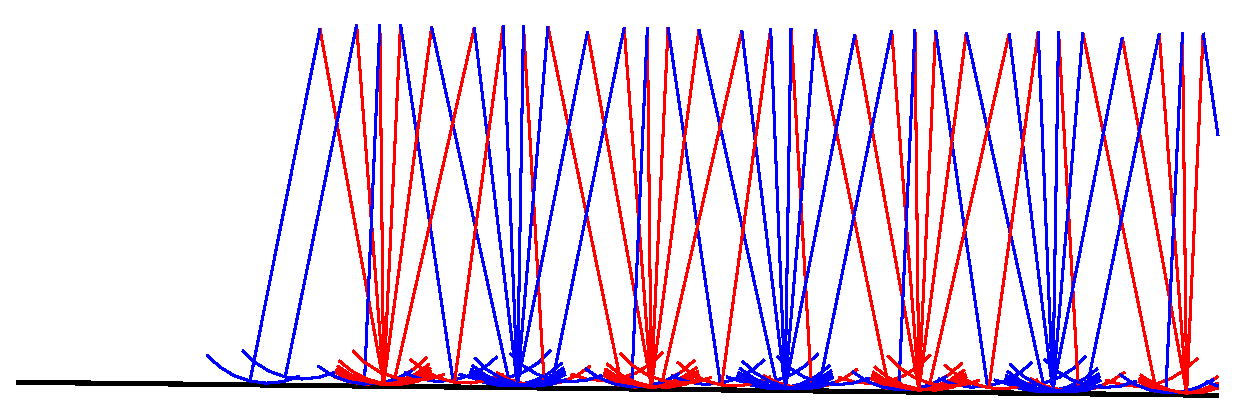
\includegraphics[width=3in]{\figurepath/passive_walking.eps}
\caption{Stable passive walking gait}
\label{fig:passive_walk}
\end{figure}
Figure \ref{fig:passive_walk} shows the gait of the passive walker. 
After coupling the neural oscillator, the basic pattern is not changed  as shown in \figurename ~\ref{fig:stable_active_walk}.

\begin{figure}[H]
\centering
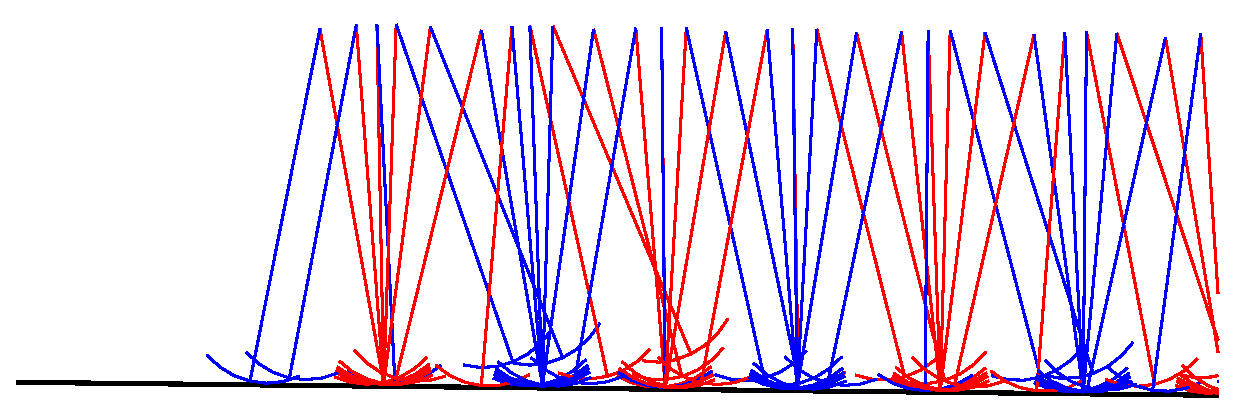
\includegraphics[width=3in]{\figurepath/actuated_walk_downslop.eps}
\caption{Walk down the same slop when actuated}
\label{fig:stable_active_walk}
\end{figure}

\textbf{Walking On Plain}
However the stability of this passive waking is fragile. The passive walker can't walk on plane. 
The step size will decrease after each step, and finally it will stop or fall over as illustrated in \figurename ~\ref{fig:pass_waling_on_plane}.
\begin{figure}[!h]
\centering
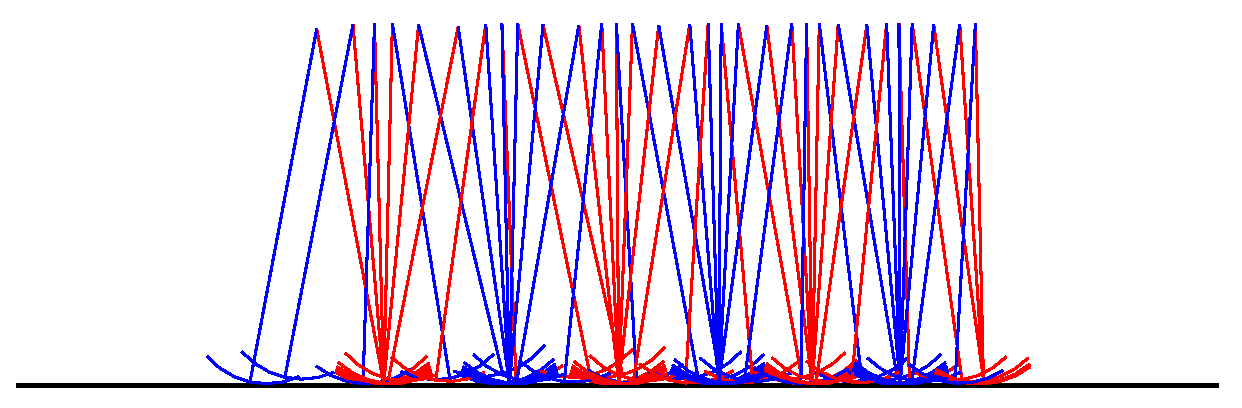
\includegraphics[width=3in]{\figurepath/passive_walk_on_plane.eps}
\caption{Passive walking gait can't be maintained on plane}
\label{fig:pass_waling_on_plane}
\end{figure}

After coupled with the neural oscillator, this walking machine can walk on plane, and exhibits gait similar to the passive dynamic walker. 
\figurename ~\ref{fig:walk_plane} shows the gait. 
From the state plot \figurename ~\ref{fig:walk_plane_state}, and phase plot \figurename ~\ref{fig:walk_plane_phase}, we can see that the gait converged to a stable limit circle.


\begin{figure}[!h]
\centering
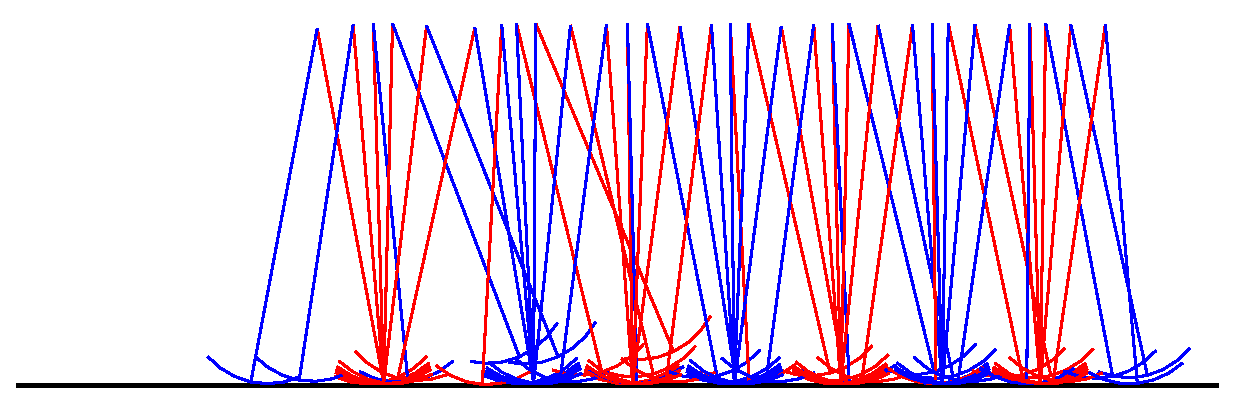
\includegraphics[width=3in]{\figurepath/walker_on_plane.eps}
\caption{Walking on plane under neural control}
\label{fig:walk_plane}
\end{figure}


\begin{figure}[!h]
\centerline{
\subfigure[State Plot]{
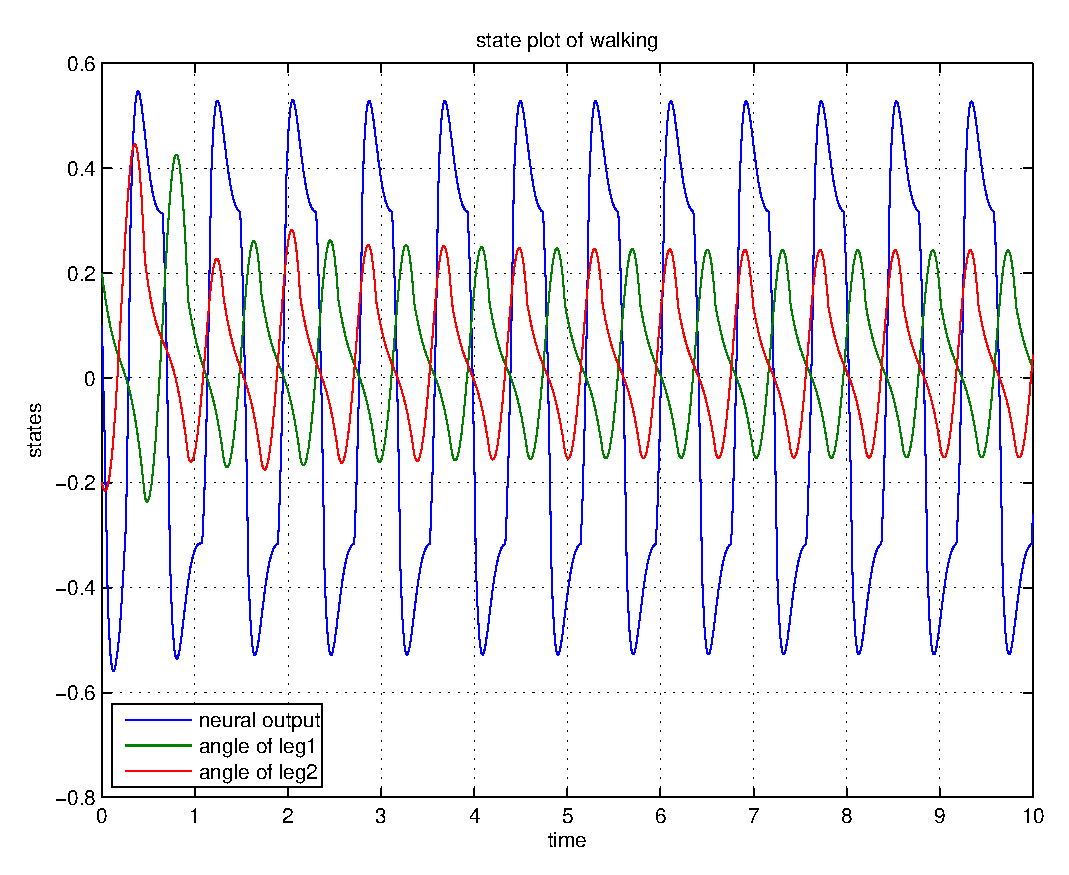
\includegraphics[width=1.5in]{\figurepath/walking_on_plane_time_state}
\label{fig:walk_plane_state}
}
\hfill
\subfigure[Phase Plot]{
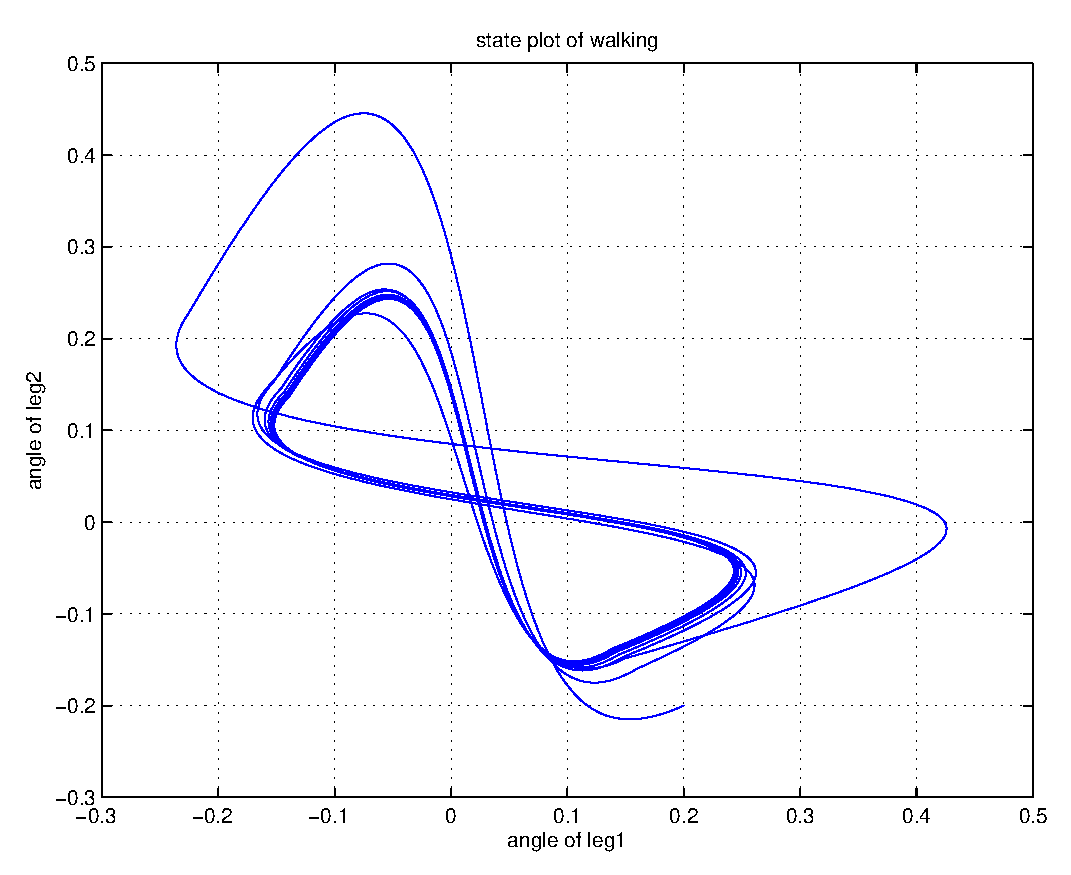
\includegraphics[width=1.5in]{\figurepath/walking_on_plane_phase.eps}
\label{fig:walk_plane_phase}
}
}
\caption{
Walking on a plane converges to a stable limited circle
}
\label{fig:walk_on_plane}
\end{figure}

\subsection{Structural stability under perturbations}
To verify the structural stability, we introduce a variety of perturbations to the passive walker. 
These perturbations include different initial condition, different slopes, different leg mass and different leg length.

\textbf{Different Initial Condition}
The original passive walker is not very stable. 
A slight change in initial condition will result in walking failure. 
While after coupled with neural oscillator, the basin of attraction has been enlarged. 
A different initial condition can still lead to a stable gait, as show in Figure \ref{fig:diff_init}. 
Natural looking gait is maintained.
\begin{figure}[h]
\centering
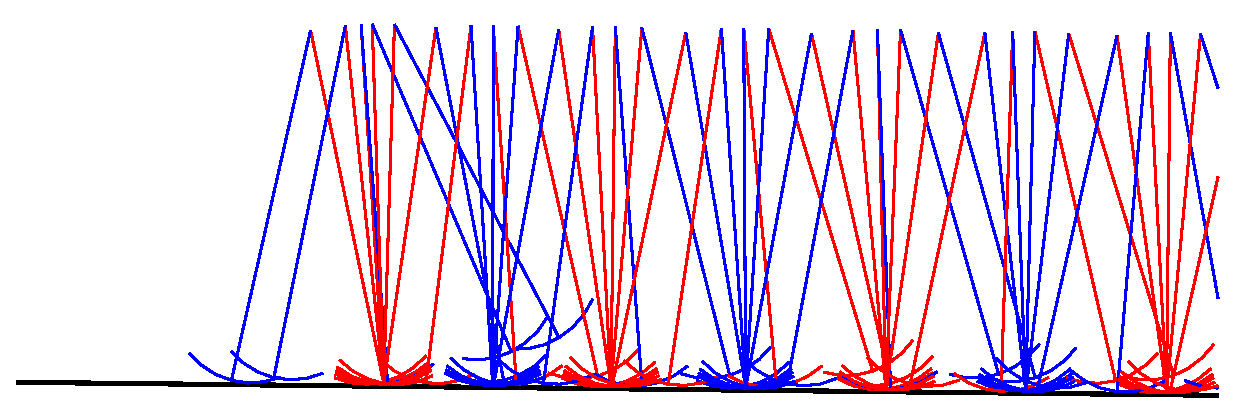
\includegraphics[width=3in]{\figurepath/walk_down_with_differnt_init_cond_suceed.eps}
\caption
{
Walking with different Initial condition
}
\label{fig:diff_init}
\end{figure}
 

\textbf{Walking On Different Slopes}
Another parameter we change is angle of the walking slope. 
When we increase the down slope, stable walking motion can still be maintained, as shown in figure \ref{fig:diff_slop}.
An important discovery is that although the walkers can walk on various down slopes, it can not walk up slope, no matter how control parameters are changed.
It can't walk up slope and will fall backward after several steps. 
We think that this is mainly because the proper limit circle does not exist in the dynamic system when walking up slope. Involving the upper body into this structure may help to solve this problem.

\begin{figure}[h]
\centering
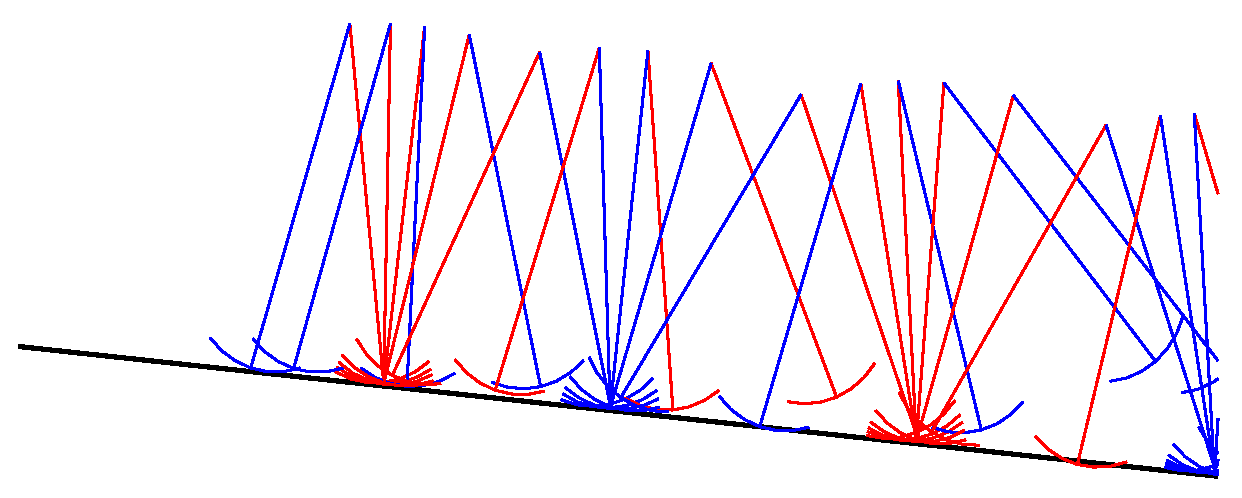
\includegraphics[width=3in]{\figurepath/big_slop_actuated_suceed.eps}
\caption
{
Walking with different slope angle
}
\label{fig:diff_slop}
\end{figure}

\textbf{Leg Mass Variation}
We add mass on one leg to 150\% and find the stability of the gait is still maintained. 
The step length and swing period of the two legs are different, this gait is similar to that with a crippled leg, see figure\ref{fig:leg mass}.

\begin{figure}[H]
\centering
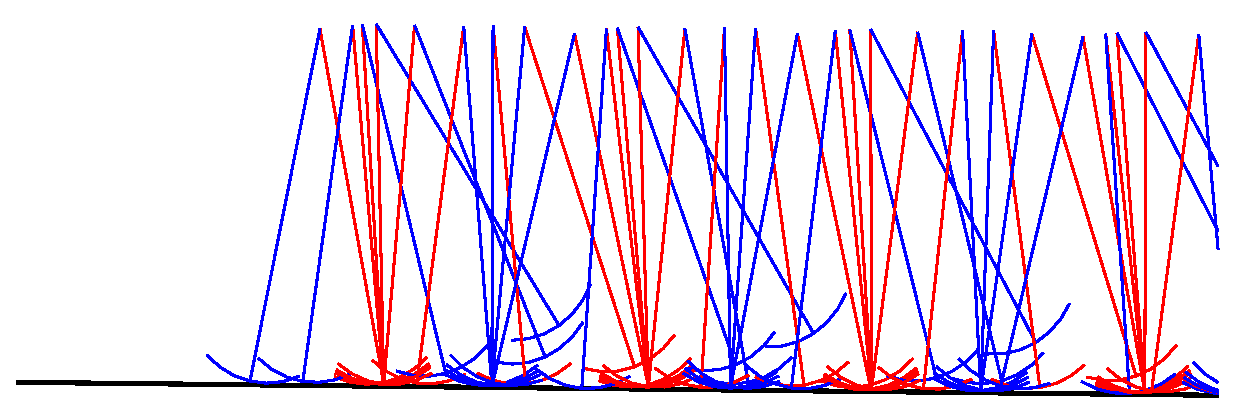
\includegraphics[width=3in]{\figurepath/walk_mass_changed.eps}
\label{fig:walk_mass_changed}
\caption
{
Walking with legs of different mass
}
\label{fig:leg mass}
\end{figure}

\textbf{Leg Length Variation}
The last parameter we change is the leg length. 
We change the leg length to 1/8 shorter. 
And we find the stability of the gait is maintained, see \figurename ~\ref{fig:walk_leg_changed}

\begin{figure}[H]
\centering
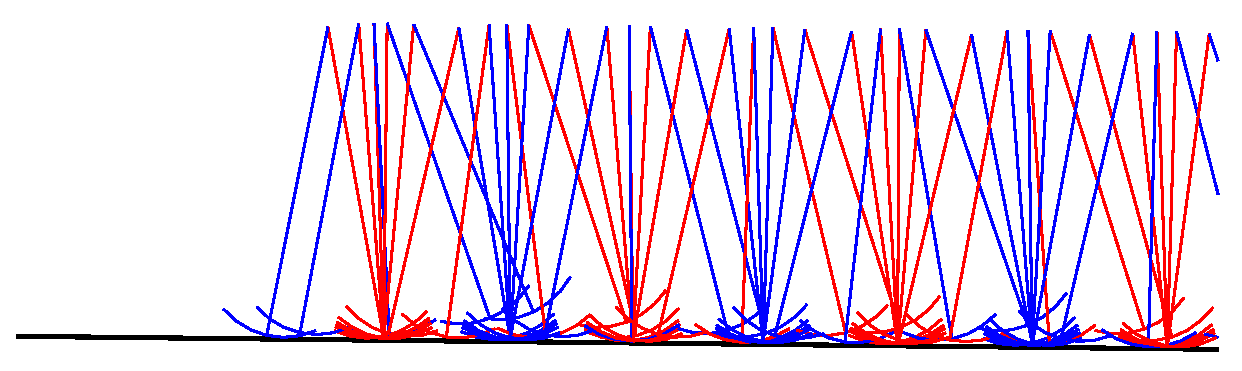
\includegraphics[width=3in]{\figurepath/walk_leg_changed_success.eps}
\caption
{
Walking with shorter Legs
}
\label{fig:walk_leg_changed}
\end{figure}

